%
%  Simulation BSP
%
%  Created by Johannes Kasberger on 2011-07-15.
\documentclass[a4paper]{article}

\usepackage[utf8]{inputenc}
\usepackage{ngerman}
\usepackage{fullpage}
\usepackage{listings}
\usepackage{color}
\usepackage{ifpdf}
\usepackage{float}
\usepackage[pdftex]{graphicx}

\title{Diskrete Regelung}
\author{Johannes Kasberger\\Markus Klein\\Simon Sperl}

\date{Juli 2011}


\definecolor{listinggray}{gray}{0.9}

\begin{document}

\lstset{language=matlab}
\lstset{backgroundcolor=\color{listinggray}}
\lstset{linewidth=120mm}
\lstset{frameround=tttt}
\lstset{keywordstyle=\color{red}\bfseries\underbar}

\maketitle

\section{Füllstandsregelung eines Viertanksystems}

Diese Aufgabe basiert auf dem Buch \emph{Modellbildung und Simulation dynamischer Systeme} von Helmut E. Scherf.

Es ist folgender Aufbau gegeben: Vier Tanks sind miteinander durch Röhren verbunden. Ein Motor pumpt Wasser in den ersten Tank und das Wasser fließt im letzten Tank ab. Der Querschnitt der Röhren ist grundsätzlich einstellbar, bleibt jedoch während des Betriebs konstant. Das Ziel ist es, den Füllstand im letzten Tank auf eine gewünschte Höhe zu regeln. Ein kontinuierlicher Regler der diese Aufgabe erfüllt, ist im Buch Modellbildung und Simulation dynamischer Systeme von H.E. Schärf beschrieben. Unsere Aufgabe ist es dieses kontinuierlichen Regler in einen diskreten Regler umzuwandeln. Das Model der Tanks haben wir vom Buch übernommen und in einen Simulink Block gekapselt. 

Der Regler ist im Buch als PID Regler ausgeführt. Um daraus einen diskreten Regler bauen zu können, muss die Übertragungsfunktion diskretisiert werden. Das geschieht mit der Matlab Funktion c2d. Wenn man die Übertragungsfunktion eines idealen Reglers so transformiert, funktioniert der digitale Regler aber nicht richtig. Es muss noch eine parasitäre Zeitkonstante zum kontinuierlichen Regler hinzugefügt werden (somit wird er zum realen PID Regler) und dieser kann dann diskretisiert werden. Diese Rechnung passiert in der Datei \emph{koef.m }. Darin werden auch alle benötigten Konstanten definiert, daher muss diese Datei ausgeführt werden um das Simulink Model lauffähig zu machen. 

\lstinputlisting[caption={koef.m für Viertanksystem}] {../bsp1/koef.m}

Um das Verhalten des diskreten und des kontinuierlichen Reglers vergleichen zu können, haben wir die Zwei gleichzeitig simuliert und die Ergebnisse in einem Plot dargestellt (Abbildung \ref{fig:bsp1}). Der Plot zeigt, dass das Verhalten der zwei Regler gut übereinstimmt. Die Abweichung der Stellgrößen der Regler beträgt maximal 3 und pendelt sonst immer um 0 (ist im mittleren Plot in Abbildung \ref{fig:bsp1}). Der Füllstand im oberen Plot und auch die Stellgrößen im unteren Plot sind weitgehend deckungsgleich.

Der diskrete Regler wurde in zwei Varianten realisiert. Einmal mit dem Simulink Block \emph{Discrete Filter} (in Datei diskre.mdl realisiert). Die Koeffizienten für diesen Filter werden in der Datei koef.m berechnet und hier verwendet. Die andere Variante (in der Datei diskr\_matlab.mdl zu finden, für Code siehe Listing \ref{fig:bsp1_code}) verwendet eine selbst geschriebene Embedded Matlab Function. Darin wird die Matlab Function \emph{filter} verwendet, um die Inputdaten zu filtern. Die Koeffizienten sind die Gleichen wie bei der Simulink Variante. Auch diese Variante stimmt gut mit dem kontinuierlichen Regler überein.

\begin{figure}[H]
    \centering
    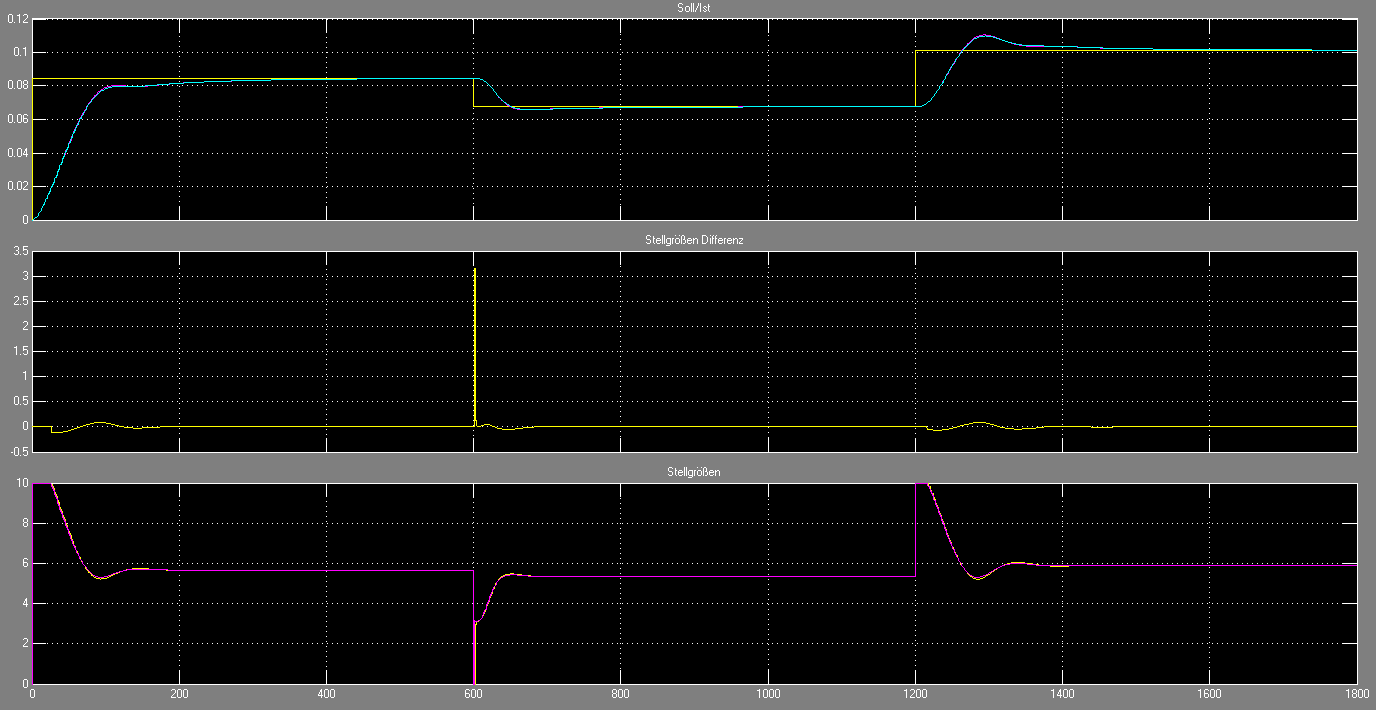
\includegraphics[width=\linewidth]{erg_bsp1.png}
    \caption{Vergleich Kontinuierlicher/Diskreter Regler für das Viertanksystem}
    \label{fig:bsp1}
\end{figure}

\lstinputlisting[caption={Code für Matlab Function für Viertanksystem},label=fig:bsp1_code] {bsp1.m}

\section{Aufheizen eines Werkstücks in einem Glühofen}

Diese Aufgabe basiert auf dem Buch \emph{Modellbildung und Simulation dynamischer Systeme} von Helmut E. Scherf.

Bei diesem Beispiel geht es um einen Glühofen in den ein Werkstück mit der Masse m und einer Ausgangstemperatur in den Ofen gelegt. Nun soll eine bestimmte Temperatur im Ofen erreicht und gehalten werden. Die Oberfläche $A$ und der Wärmeübergangskoeffizient $\alpha$ des Werkstücks sind bekannt. Im Buch wird ausgeführt wie die Differentialgleichungen aufgestellt werden müssen. Dabei lassen sich alle Variablen die das Werkstück beschreiben in die Formel $T= \frac{c m}{\alpha A}$ zusammen fassen. Dieser Gleichung die die Temperatur ($\vartheta_G$) im Ofen beschreibt ist $T*\dot{\vartheta_W}+\vartheta_W = \vartheta_G$. Die Temperatur des Werkstückes wird mit $\vartheta_W$ bezeichnet. 

Diese Differentialgleichung wurde im Buch als kontinuierlicher Regler realisiert. Wie im ersten Beispiel auch haben wir auch hier die Übertragungsfunktion diskretisiert. Hier haben wir verschiedene Optionen der c2d Funktion ausprobiert und die Ergebnisse vergleichen (siehe Abbildung \ref{fig:reg_bsp2}). Wir haben hier die Algorithmen Zero Order Hold, Triangle approximation und Impulse invariant discretization verwendet. Die Ergebnisse der verschiedenen Algorithmen sind in der Abbildung \ref{fig:bsp2} zu sehen. Die Abweichung zum kontinuierlichen Regler ist mit allen Diskreten Reglern sehr klein.

Auch hier wurde der Regler einmal als Simulink und einmal als Embedded Matlab Function realisiert. Der Code für die Embedded Matlab Function ist im Listing \ref{code:bsp2} angegeben.

\begin{lstlisting}[caption={Code für Matlab Function für Glühofen},label=code:bsp2]
    function tmp = PI(wert,T,step)
        persistent X

        if isempty(X)
            X = 0;
        end

        X = X + wert/T*step;
        tmp = X;
\end{lstlisting}

\begin{figure}[H]
    \centering
    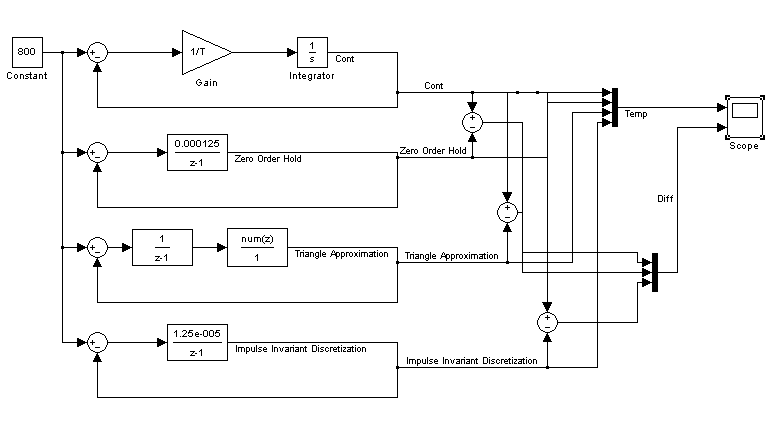
\includegraphics[width=\linewidth]{regler_bsp2.png}
    \caption{Implementierung der Regler für den Glühofen}
    \label{fig:reg_bsp2}
\end{figure}

\begin{figure}[H]
    \centering
    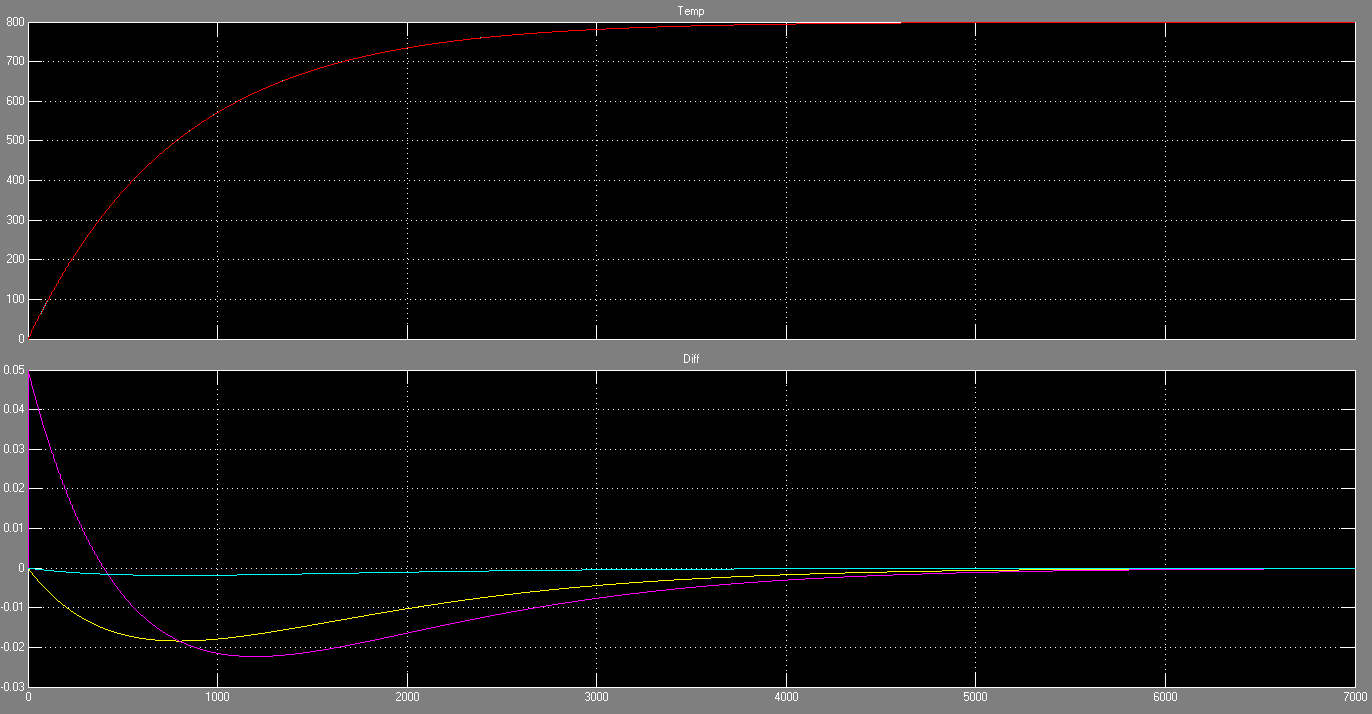
\includegraphics[width=\linewidth]{erg_bsp2.png}
    \caption{Vergleich Kontinuierlicher/Diskreter Regler für den Glühofen}
    \label{fig:bsp2}
\end{figure}

\section{Fahrradmodell}

Aufgabe war die Implementierung und Regelung eines vereinfachten Fahrradmodells (Eyckhoff, 1974).

\begin{eqnarray}
z_1 & =& Lenkausschlag \\
z_2 & =& Fahrerneigung \\
p & =& Fahrradneigung \\
dmv\dot{z_1} + mv^2z_1 & = & J\ddot{p} - mhgp + (J* + h^2m)\ddot{z_2} - 1/2mgz_2 
\end{eqnarray}

In Worten bedeuted die Formel:

Gyroskopisches Moment des Vorderrads + Zentrifugalmoment der Gesamtmasse= Trägheitsmoment des Fahrrads - Gravitationsmoment des Fahrrads + Trägheitsmoment des Fahrers - Gravitationsmoment des Fahrers

\paragraph*{}
Für die Parameterstudie verwenden wir realistische Werte:

\begin{tabular}{ccccc}
 g          & v         & $m_{bike}$  & $m_{biker}$    & h     \\ 
 $9.81 m/s^2$ & $3 m/s$ & $5 kg$      & $50 kg$        & $0.9 m$   
\end{tabular} 
siehe \textit{koeff.m} 


\paragraph*{}
W\"ahrend der Studie war es wichtig zu beachten das für $z_i,z_2,p$, wegen der mehrmals gew\"ahlte Vereinfachung $sin(z_1)\approx z_1$, nur Werte im Bereich $ [ -\frac{\pi}{4},  \frac{\pi}{4}]$  angenommen werden.
F\"ur die Simulation bedeuted dies: wenn Fahrer oder Fahrrad zu stark geneigt sind, dann ist kein realistisches Verhalten mehr zu erwarten.

Die Angabe verwendet nun zwei PID Regler zur Steuerung von $z_1$ und $z_2$ um p wieder in Ausgangslage zu bringen. 
Pers\"onlich w\"urde eine Regelung von $z_2$ abh\"angig von Lenkausschlag $z_1$ und Momentangeschwindigkeit $v$ die es vermeidet das \textit{man hinfällt}.
Im Sinne von Je schneller ich fahre und je enger die Kurve desto mehr muss ich mich reinlegen.

Bei einer kontinuerlichen Störung des Lenkauschlags $z_1$ mittels einer schwachen Sinusschwingung Amplitude $0.05 rad$ und Frequenz $0.2 Hz$, und allen Parametern der PID-Regler auf 0.0001 bleibt das Fahrrad stabil.
Wobei sich $K_i$ im Bereich von 0.05 bis 0.0001 bewegen darf, die $K_p$ und $K_d$ sind wesentlich empfindlicher.
Die Vereinfachung von $sin(x) = x$ für kleine x hat sich für die Parameterstudie als stark problematisch herausgestellt, da sie den Übergang zwischen etwas falschen und völlig falschen Parametern stark verkleinert.

Das Ergebnis des Parameterstudie ist im großen und ganzen sch\"on gleichm\"asige St\"orungen und ganz vorsichtig den K\"orper neigen dann geht im Modell alles gut.

\begin{figure}[ht!]
    \centering
    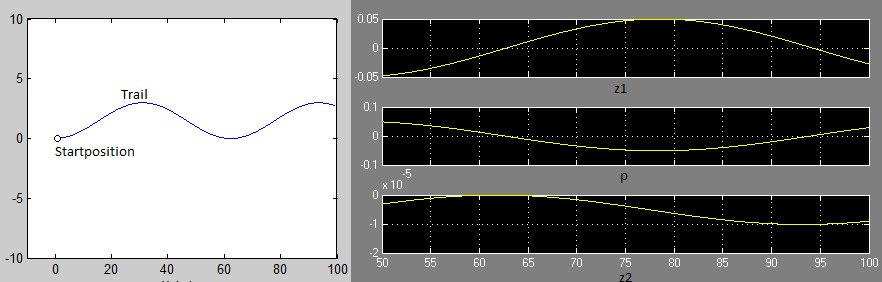
\includegraphics[width=\linewidth]{erg_bsp3.png}
    \caption{Testfahrt, mit sinusartig st\"orschlingenden Lenker, \textit{siehe Fahrrad2.sim}}
    \label{fig:bsp3}
\end{figure}


\begin{figure}[ht!]
    \centering
    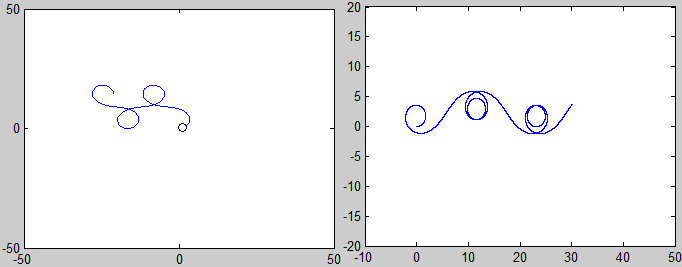
\includegraphics[width=\linewidth]{bsp3_goof.png}
    \caption{H\"ubsche Fahrradfahrten, erzeugt durch veränderte Frequenzen und Amplituden der Störschwingungen}
    \label{fig:bsp3goof}
\end{figure}



\end{document}
